\documentclass[t]{beamer}
\usetheme{Copenhagen}
\setbeamertemplate{headline}{} % remove toc from headers
\beamertemplatenavigationsymbolsempty

\usepackage{amsmath, tikz, pgfplots}
\pgfplotsset{compat = 1.16}
%\usetkzobj{all}

\title{Factoring Techniques}
\author{}
\date{}

\AtBeginSection[]
{
  \begin{frame}
    \frametitle{Objectives}
    \tableofcontents[currentsection]
  \end{frame}
}

\begin{document}

\begin{frame} 
\maketitle
\end{frame}

\section{Find the greatest common factor of a quadratic expression.}

\begin{frame}{Greatest Common Factor}
The \alert{greatest common factor}, or GCF, of an expression is the largest term that divides into each term of that expression.	\newline\\	\pause

To find the greatest common factor of an expression:	\newline\\	\pause
\begin{itemize}
	\item Find the greatest common factor of the coefficients.	\newline\\	\pause
	\item Select the \underline{lowest power} of each unique variable.	\newline\\	\pause
\end{itemize}

Then divide each term by that GCF.
\end{frame}

\begin{frame}{Example 1}
Factor the GCF from each.	\newline\\
(a) \quad $16x^5 + 72x^3 - 36x^2$		\newline\\	\pause
GCF of 16, 72, and 36 is 4	\newline\\	\pause
Lowest power of $x$ is 2, so the GCF of the variables is $x^2$	\newline\\	\pause
GCF is $4x^2$	\newline\\	\pause
\[4x^2\left(4x^3+18x-9\right)\]
\end{frame}

\begin{frame}{Example 1}
(b) \quad $5a^4 + 70a^2 - 25a$ \newline\\ \pause
GCF of 5, 70, and 25 is 5 \newline\\	\pause
Lowest power of $a$ is 1, so the GCF of the variables is $a$ \newline\\ \pause
GCF is $5a$ \newline\\ \pause
\[5a\left(a^3+14a-5\right)\]
\end{frame}

\section{Factor trinomials in the form $x^2+bx+c$}

\begin{frame}{$x^2+bx+c$}
When factoring trinomials in the form $x^2+bx+c$, we are looking to find 2 numbers that {\color{blue}\textbf{multiply}} to make $c$ and {\color{red}\textbf{add}} to make $b$.	\newline\\	\pause

We can then write the factorization in the form
\[ (x+m)(x+n) \]
where $mn = c$ and $m+n=b$
\end{frame}

\begin{frame}{Example 2}
Factor each completely.	\newline\\
(a) \quad $x^2 + 15x + 36$	\newline\\
\onslide<2->{Product of the two numbers is 36.} \newline\\
\onslide<3->{Sum of the two numbers is 15.} \newline\\
\onslide<4->{Numbers are 3 and 12} \newline\\
\onslide<5->{\[(x+3)(x+12)\]}
\end{frame}

\begin{frame}{Visual Approach to Factoring}
$x^2 + 15x + 36$	\newline\\	
\onslide<2->{
\begin{center}
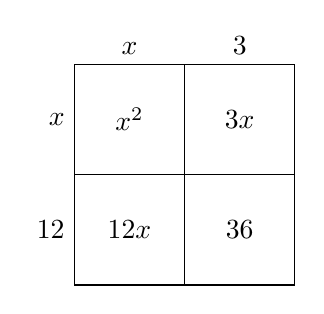
\begin{tikzpicture}[scale=0.7]
\draw (0,0) rectangle (4,4);
\draw (0,2) -- (4,2);
\draw (2,0) -- (2,4);
\onslide<3->{\node at (1,3) {$x^2$};}
\onslide<4->{\node at (0,3) [left] {$x$}; \node at (1,4) [above] {$x$};}
\onslide<5->{\node at (3,1) {$36$};}
\onslide<6->{\node at (3,4) [above] {3}; \node at (0,1) [left] {12};}
\onslide<7->{\node at (1,1) {$12x$}; \node at (3,3) {$3x$};}
\end{tikzpicture}
\end{center}	}
\onslide<8->{\[(x+3)(x+12)\]}
\end{frame}

\begin{frame}{Example 2}
(b) \quad $x^2 - 9x + 14$ \newline\\
\onslide<2->{Product of the two numbers is 14.} \newline\\
\onslide<3->{Sum of the two numbers is $-9$.} \newline\\
\onslide<4->{Numbers are $-7$ and $-2$} \newline\\
\onslide<5->{\[(x-7)(x-2)\]}
\end{frame}

\begin{frame}{Example 2}
(c) \quad $x^2+ 5x - 6$ \newline\\
\onslide<2->{Product of the two numbers is $-6$.} \newline\\
\onslide<3->{Sum of the two numbers is 5.} \newline\\
\onslide<4->{Numbers are $-1$ and 6} \newline\\
\onslide<5->{\[(x-1)(x+6)\]}
\end{frame}

\begin{frame}{Example 2}
(d) \quad $x^2 - 7x - 8$ \newline\\
\onslide<2->{Product of the two numbers is $-8$.} \newline\\
\onslide<3->{Sum of the two numbers is $-7$.} \newline\\
\onslide<4->{Numbers are $-8$ and 1} \newline\\
\onslide<5->{\[(x-8)(x+1)\]}
\end{frame}

\section{Factor trinomials in the form $ax^2+bx+c$}

\begin{frame}{$ax^2 + bx + c$}
To factor quadratic expressions in the form $ax^2+bx+c$, we will first \alert{transform} them into the form $x^2+bx+c$ by {\color{blue}\textbf{multiplying}} the values of $a$ and $c$ to get:	\newline\\	\pause

\[x^2 + bx + ac\]	\pause

We can then factor like in the last example, but we will have to remember to \textbf{transform the expression back}; as we will see.
\end{frame}

\begin{frame}{Example 3}
Factor each completely.	\newline\\
(a) \quad $3x^2 - 11x - 4$	\newline\\	
\onslide<2->{Multiply $a=3$ and $c=-4$ to get $ac=-12$.}	\newline\\
\onslide<3->{Factor $x^2 - 11x - 12$}
\onslide<4->{\[(x-12)(x+1)\]}
\begin{center}
\onslide<5->{\Huge{\color{red}\textbf{We are not done yet!!}}}
\end{center}
\end{frame}

\begin{frame}{Example 3 \quad $3x^2 - 11x - 4$}
\[(x-12)(x+1)\]
\onslide<2->{Divide the $-12$ and $1$ by {\color{blue}\textbf{3}} and simplify.} 
\onslide<3->{\[\left(x-\frac{12}{3}\right)\left(x+\frac{1}{3}\right)\]}	
\onslide<4->{\[\left(x-4\right)\left(x+\frac{1}{3}\right)\]}	
\onslide<5->{Slide any remaining denominators in front of their variable.}
\onslide<6->{\[(x-4)(3x+1)\]}
\end{frame}

\begin{frame}{Example 3}
(b) \quad $8x^2 + 2x - 3$ \newline\\
\onslide<2->{Multiply $a=8$ and $c=-3$ to get $ac=-24$}	\newline\\
\onslide<3->{Factor $x^2 + 2x - 24$}
\onslide<4->{\[(x+6)(x-4)\]}
\onslide<5->{\[\left(x + \frac{6}{8}\right)\left(x-\frac{4}{8}\right)\]}
\onslide<6->{\[\left(x + \frac{3}{4}\right)\left(x-\frac{1}{2}\right)\]}
\onslide<7->{\[(4x+3)(2x-1)\]}
\end{frame}

\begin{frame}{Example 3}
(c) \quad $16x^2 + 46x + 15$	\newline\\
\onslide<2->{Multiply $a=16$ and $c=15$ to get $ac=240$} \newline\\
\onslide<3->{Factor $x^2 + 46x + 240$}
\onslide<4->{\[(x+40)(x+6)\]}
\onslide<5->{\[\left(x+\frac{40}{16}\right)\left(x+\frac{6}{16}\right)\]}
\onslide<5->{\[\left(x+\frac{5}{2}\right)\left(x+\frac{3}{8}\right)\]}
\onslide<6->{\[(2x+5)(8x+3)\]}
\end{frame}

\begin{frame}{Example 3}
(d) \quad $7x^2 - 55x + 42$	\newline\\
\onslide<2->{Multiply $a=7$ and $c=42$ to get $ac=294$} \newline\\
\onslide<3->{Factor $x^2 - 55x + 294$}
\onslide<4->{\[(x-49)(x-6)\]}
\onslide<5->{\[\left(x-\frac{49}{7}\right)\left(x-\frac{6}{7}\right)\]}
\onslide<5->{\[\left(x-7\right)\left(x-\frac{6}{7}\right)\]}
\onslide<6->{\[(x-7)(7x-6)\]}
\end{frame}

\section{Use ``reverse engineering" to factor quadratic expressions}

\begin{frame}{Using the Graph}
You can also use the $x$-intercepts of the graph of the quadratic expression to help you factor.	\newline\\	\pause

For instance, the graph for $x^2 + 5x - 6$ has $x$-intercepts at $x=-6$ and $x=1$.	

\begin{align*}
\onslide<3->{x &= -6 & x&= 1} \newline\\
\onslide<4->{x+6&=0 & x-1&= 0} \newline\\
\end{align*}
\begin{center}
\onslide<5->{$x^2+5x-6$ factors as $(x+6)(x-1)$}
\end{center}
\end{frame}

\begin{frame}{Using the Graph for $ax^2 + bx + c$}
For expressions in the form $ax^2 + bx + c$:	\newline\\	\pause
\begin{enumerate}
	\item<+-> Get the transformation expression by multiplying $a$ and $c$.	\newline\\
	\item<+-> Find those $x$-intercepts \newline\\
	\item<+-> Transform back by dividing by the value of $a$ and simplifying like in Example 3.
\end{enumerate}
\end{frame}

\begin{frame}{Using the Graph for $ax^2 + bx + c$}
For instance, we transformed $3x^2 - 11x - 4$ to $x^2 -11x - 12$	\newline\\	\pause
The $x$-intercepts of $x^2-11x-12$ are $x=-1$ and $x=12$	\newline\\	\pause
Divide each of those by 3 to get $x=-\frac{1}{3}$ and $x=4$ \pause	\newline\\
Move any remaining denominators in front of their variable: \pause \[3x=-1 \quad  \text{and} \quad x=4\] 	\pause
Get each equal to 0: \pause
\[3x+1 \quad \text{and} \quad x-4\]		\pause
\[(3x+1)(x-4)\]
\end{frame}

\end{document}